\chapter{Implementasi dan Pengujian}
Pada bab ini, akan dibahas hasil dari implementasi dan pengujian terhadap perangkat lunak yang dibangun. Terdapat spesifikasi lingkungan perangkat lunak dan perangkat keras yang digunakan dalam melakukan implementasi dan pengujian.
%Terdapat 2 jenis pengujian yang dilakukan, yaitu pengujian fungsional dan pengujian eksperimental.

\section{Lingkungan Implementasi Perangkat Keras}
Berikut ini merupakan spesifikasi perangkat keras yang digunakan baik pada tahap implementasi maupun pada tahap pengujian:
\begin{itemize}
	\item CPU: Intel\textsuperscript{\textregistered}{ }Core\texttrademark{ }i5-7200U Processor, 3M Cache, up to 3.10 Ghz
	\item GPU: NVIDIA GeForce 930MX
	\item RAM: 8GB
\end{itemize}

\section{Lingkungan Implementasi Perangkat Keras}
Berikut ini merupakan spesifikasi perangkat lunak yang digunakan baik pada tahap implementasi maupun pada tahap pengujian:
\begin{itemize}
	\item OS: Windows 10 Pro, 64-bit
	\item Pemrograman: Java 8 Update 152 (64-bit)
\end{itemize}

\section{Implementasi Antarmuka}
Pada bagian ini, akan dibahas hasil implementasi antarmuka sesuai dengan perancangan antarmuka yang dilakukan pada~\ref{sec:perancangan_antarmuka}. Berikut ini merupakan hasil implementasi antarmuka:
\begin{itemize}
	\item Antarmuka: \textbf{Penerima Masukan}\\
	Gambar~\ref{fig:ui_input} menunjukkan tampilan antarmuka penerima masukan. Pada antarmuka ini terdapat kolom-kolom masukan yang dapat diisi oleh pengguna. Apabila pengguna telah yakin dengan masukan yang diberikan, pengguna dapat menekan tombol ''\textit{submit}'' untuk diarahkan ke antarmuka penempatan kamera CCTV.
	\begin{figure}[H]
		\centering  
		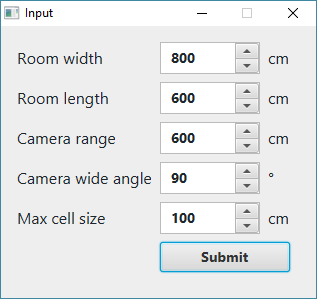
\includegraphics[scale=0.6]{ui_input}
		\caption[Antarmuka penerima masukan]{Antarmuka penerima masukan}
		\label{fig:ui_input}
	\end{figure}
	
	\item Antarmuka: \textbf{Penempatan Kamera CCTV}\\
	Gambar~\ref{fig:ui_simulator} menunjukkan tampilan antarmuka penempatan kamera CCTV. Pada antarmuka ini, pengguna dapat melihat solusi penempatan-penempatan kamera CCTV berdasarkan masukan yang telah dimasukkan sebelumnya. Pada bagian kiri terdapat informasi mengenai spesifikasi masalah uang terdiri dari spesifikasi ruangan dan spesifikasi kamera CCTV. Selain itu, terdapat informasi lainnya seperti ukuran matriks \textit{cell}, ukuran \textit{cell}, tingkat ketercakupan, dan tingkat \textit{overlap out of bound}. Pada bagian kanan terdapat visualisasi penempatan kamera CCTV dalam ruangan yang dipecah menjadi matriks \textit{cell}.
	\begin{figure}[H]
		\centering  
		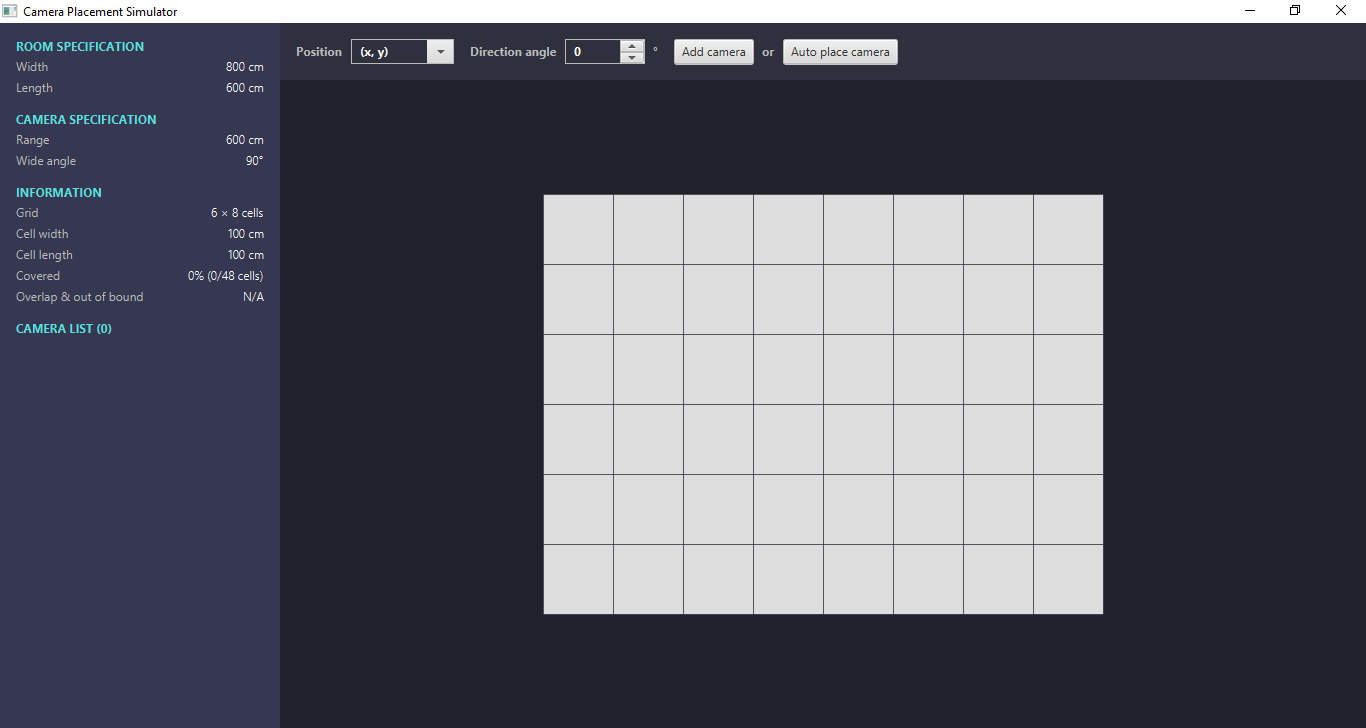
\includegraphics[scale=0.45]{ui_simulator}
		\caption[Antarmuka penempatan kamera CCTV]{Antarmuka penempatan kamera CCTV}
		\label{fig:ui_simulator}
	\end{figure}
\end{itemize}

\section{Pengujian}
Pada perangkat lunak yang telah dibangun, akan dilakukan 2 buah pengujian. Pengujian pertama dilakukan untuk melihat pengaruh perubahan masukan terhadap ukuran masalah masalah \textit{binary integer programming}. Pengujian kedua dilakukan untuk membandingkan jumlah iterasi pada algoritma \textit{Balas's additive} dengan iterasi \textit{exhaustive search} berjumlah \(2^n\).

\subsection{Pengujian-1}
Pada pengujian ini, akan dilihat pengaruh perubahan masukan masalah terhadap ukuran masalah \textit{binary integer programming}. Sebanyak 4 buah eksperimen akan dilakukan dalam pengujian ini. Masukan yang digunakan untuk eksperimen ini dibagi menjadi 2 bagian:
\begin{itemize}
	\item \textbf{Masukan tetap}\\
	\begin{tabular}{ll}
		- Jarak pandang kamera CCTV &: 100 cm\\
		- Sudut pandang kamera CCTV &: $90^\circ$\\
		- Ukuran terbesar \textit{cell} &: 50 cm\\
		- Jumlah kemungkinan arah pandang kamera CCTV &: 8 buah\\
	\end{tabular}
	\item \textbf{Masukan tidak tetap}\\
	\begin{tabular}{ll}
		- (Eksperimen-1) Ukuran ruangan &: 100 cm $\times$ 100 cm\\
		- (Eksperimen-2) Ukuran ruangan &: 100 cm $\times$ 150 cm\\
		- (Eksperimen-3) Ukuran ruangan &: 150 cm $\times$ 150 cm\\
		- (Eksperimen-4) Ukuran ruangan &: 200 cm $\times$ 150 cm\\
	\end{tabular}
\end{itemize}
Berdasarkan masukan tersebut didapatkan informasi sebagai berikut:
\begin{itemize}
	\item \textbf{Informasi}\\
	\begin{tabular}{ll}
		- (Eksperimen-1) Matriks \textit{cell} &: 2 $\times$ 2 = 4 \textit{cells}\\
		- (Eksperimen-2) Matriks \textit{cell} &: 3 $\times$ 2 = 6 \textit{cells}\\
		- (Eksperimen-3) Matriks \textit{cell} &: 3 $\times$ 3 = 9 \textit{cells}\\
		- (Eksperimen-4) Matriks \textit{cell} &: 4 $\times$ 3 = 12 \textit{cells}\\
	\end{tabular}
\end{itemize}
Matriks \textit{cell} didapatkan berdasarkan masukan ukuran ruangan dan masukan ukuran terbesar \textit{cell}.

\begin{figure}[H]
	\centering
	\begin{tikzpicture}
	\begin{axis}[xlabel= \textit{cells}, ylabel=Jumlah variabel (\(n\)), legend pos = outer north east]
	\addplot[smooth][color=blue,mark=*] coordinates {(4,28) (6,44) (9,68) (12, 92)};
	\end{axis}
	\end{tikzpicture}
	\caption[Diagram hubungan jumlah \textit{cells} terhadap jumlah variabel]{Diagram hubungan jumlah \textit{cells} terhadap jumlah variabel}
	\label{fig:pengujian_1}
\end{figure}

Berdasarkan eksperimen yang dilakukan, didapatkan hubungan jumlah \textit{cells} terhadap jumlah variabel (\(n\)) yang dapat dilihat pada gambar~\ref{fig:pengujian_1}. Jumlah variabel (\(n\)) merupakan jumlah kemungkinan penempatan kamera CCTV. Apabila ukuran ruangan semakin besar, maka ukuran matriks \textit{cell} akan semakin besar. Apabila matriks \textit{cell} semakin besar, maka akan titik penempatan kamera CCTV semakin banyak sehingga kemungkinan penempatan kamera CCTV juga akan semakin banyak. Dengan demikian, dapat disimpulkan bahwa apabila ukuran ruangan semakin besar, maka kemungkinan penempatan kamera CCTV juga akan semakin banyak.

\subsection{Pengujian-2}
Pada~\ref{balas_additive} diketahui bahwa pencarian solusi menggunakan algoritma \textit{Balas's additive} dilakukan secara efisien tanpa melibatkan \textit{exhaustive search}. Dengan menggunakan algoritma \textit{Balas's additive}, solusi optimal masalah \textit{binary integer programming} dapat ditemukan tanpa memeriksa seluruh \(2^n\) kemungkinan solusi di mana \(n\) menunjukkan jumlah variabel. Untuk menguji hal tersebut, akan dilakukan eksperimen perbandingan antara jumlah iterasi pada algoritma \textit{Balas's additive} dengan iterasi \textit{exhaustive search} yang berjumlah \(2^n\). Eksperimen ini dilakukan sebanyak 5 kali. Masukan yang digunakan untuk eksperimen ini dibagi menjadi 2 bagian:
\begin{itemize}
	\item \textbf{Masukan tetap}\\
	\begin{tabular}{ll}
		- Ukuran \textit{cell} &: 100 cm $\times$ 100 cm\\
		- Jarak pandang kamera CCTV &: 100 cm\\
		- Sudut pandang kamera CCTV &: $90^\circ$\\
		- Ukuran terbesar \textit{cell} &: 50 cm\\
	\end{tabular}
	
	\item \textbf{Masukan tidak tetap}\\
	\begin{tabular}{ll}
		- (Eksperimen-1) Jumlah kemungkinan arah pandang kamera CCTV &: 2 buah\\
		- (Eksperimen-2) Jumlah kemungkinan arah pandang kamera CCTV &: 4 buah\\
		- (Eksperimen-3) Jumlah kemungkinan arah pandang kamera CCTV &: 8 buah\\
		- (Eksperimen-4) Jumlah kemungkinan arah pandang kamera CCTV &: 12 buah\\
		- (Eksperimen-5) Jumlah kemungkinan arah pandang kamera CCTV &: 16 buah\\
	\end{tabular}
\end{itemize}
Berdasarkan masukan tersebut didapatkan informasi sebagai berikut:
\begin{itemize}
	\item \textbf{Informasi}\\
	\begin{tabular}{ll}
		- (Eksperimen-1) Jumlah kemungkinan penempatan kamera CCTV &: 6 buah\\
		- (Eksperimen-2) Jumlah kemungkinan penempatan kamera CCTV &: 12 buah\\
		- (Eksperimen-3) Jumlah kemungkinan penempatan kamera CCTV &: 28 buah\\
		- (Eksperimen-4) Jumlah kemungkinan penempatan kamera CCTV &: 44 buah\\
		- (Eksperimen-5) Jumlah kemungkinan penempatan kamera CCTV &: 68 buah\\
	\end{tabular}
\end{itemize}
Setiap kemungkinan penempatan kamera CCTV merupakan variabel pada model masalah \textit{binary integer programming} sehingga jumlah kemungkinan penempatan kamera CCTV menunjukkan jumlah variabel~(\(n\)).
\begin{figure}[H]
	\centering
	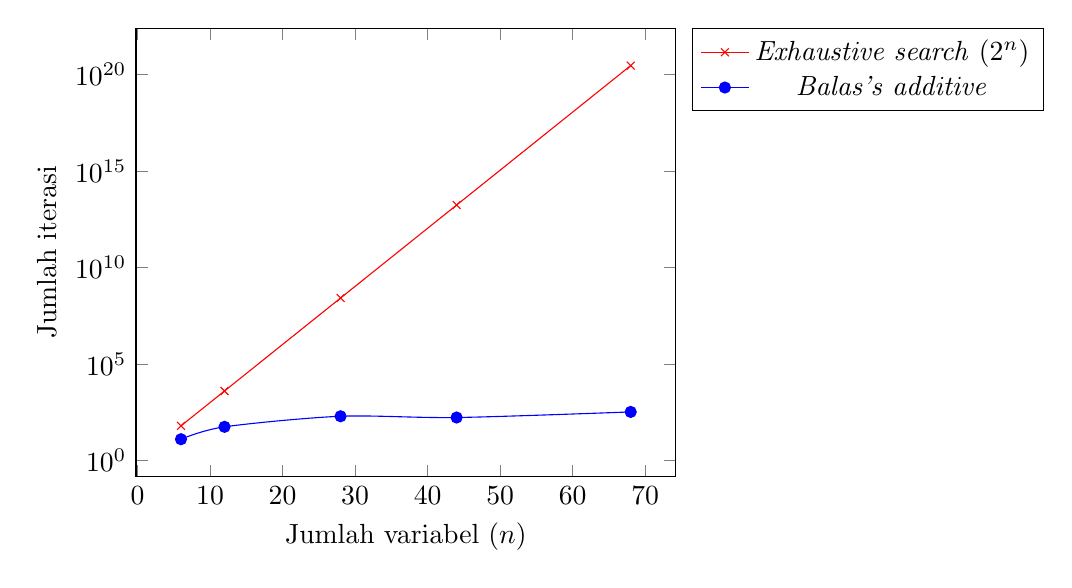
\begin{tikzpicture}
	\begin{semilogyaxis}[xlabel= Jumlah variabel (\(n\)),ylabel=Jumlah iterasi, legend pos = outer north east]
	\addplot[smooth][color=red,mark=x] coordinates {(6,64) (12,4096) (28,2.684355E8) (44, 1.759219E13) (68, 2.951479E20)};
	\addplot[smooth][color=blue,mark=*] coordinates {(6,13) (12,57) (28,201) (44, 173) (68, 337)};
	\legend{\textit{Exhaustive search} (\(2^n\)), \textit{Balas's additive}}
	\end{semilogyaxis}
	\end{tikzpicture}
	\caption[Diagram perbandingan jumlah iterasi antara \textit{Balas's additive} dengan \textit{exhaustive search}~(\(2^n\))]{Diagram perbandingan jumlah iterasi antara \textit{Balas's additive} dengan \textit{exhaustive search}~(\(2^n\))}
	\label{fig:pengujian_2}
\end{figure}

Berdasarkan eksperimen yang dilakukan, didapatkan diagram perbandingan jumlah iterasi yang dapat dilihat pada gambar~\ref{fig:pengujian_2}. Terlihat bahwa jumlah iterasi pada algoritma \textit{Balas's additive} lebih kecil dibandingkan dengan iterasi pada \textit{exhaustive search} yang berjumlah \(2^n\). Berdasarkan perbandingan tersebut, dapat disimpulkan bahwa algoritma \textit{Balas's additive} dapat menemukan solusi optimal masalah \textit{binary integer programming} secara efisien tanpa memeriksa seluruh \(2^n\) kemungkinan solusi.

%\section{Pengujian Perangkat Lunak}
%Perangkat lunak yang telah diimplementasikan perlu diuji terlebih dahulu agar berjalan sebagaimana mestinya. Pada bagian ini akan dibahas 2 jenis pengujian yang dilakukan, yaitu pengujian fungsional dan pengujian metode penyelesaian masalah. Pada pengujian fungsional, perangkat lunak akan diuji agar bekerja sesuai fungsinya. Pada pengujian metode penyelesaian masalah, perangkat lunak akan diuji dengan eksperimen-eksperimen masalah untuk memastikan perangkat lunak dapat menyelesaikan masalah.

%\section{Pengujian Fungsional}1
%Pada bagian ini, perangkat lunak akan diuji untuk memastikan bahwa setiap fungsi-fungsi dalam perangkat lunak dapat bekerja sesuai tujuannya. Pengujian ini dilakukan sesuai dengan skenario-skenario yang terdapat pada use case. Berikut ini pengujian-pengujian fungsional yang dilakukan:
%
%\begin{itemize}
%	\item Pengujian: \textbf{Memasukkan Spesifikasi Masalah}\\
%	Pada pengujian ini, akan diuji apakah perangkat lunak dapat membangun simulasi masalah yang sesuai dengan masukan yang diberikan oleh pengguna. Pada pengujian ini, akan digunakan masukan sebagai berikut:	
%	
%	\begin{itemize}
%		\item Lebar ruangan: 800 cm
%		\item Panjang ruangan: 600 cm
%		\item Jarak pandang kamera CCTV: 600 cm
%		\item Besar sudut pandang kamera CCTV: \(90^\circ\)
%		\item Ukuran terbesar cell: 100 cm
%	\end{itemize}
%
%	Masukan-masukan tersebut dimasukkan melalui antarmuka penerima masukan seperti pada gambar~\ref{fig:testing_input_before}.
%	
%	\begin{figure}[H]
%		\centering  
%		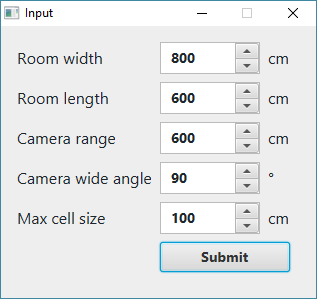
\includegraphics[scale=0.6]{ui_input}
%		\caption[Tampilan pengisian masukan masalah]{Tampilan pengisian masukan masalah}
%		\label{fig:testing_input_before}
%	\end{figure}
%	
%	Setelah masukan-masukan tersebut dimasukkan, tombol ''\textit{submit}'' ditekan. Kemudian, perangkat lunak menampilkan antarmuka simulasi penempatan kamera CCTV seperti pada gambar~\ref{fig:testing_input_after}. 
%	
%	\begin{figure}[H]
%		\centering  
%		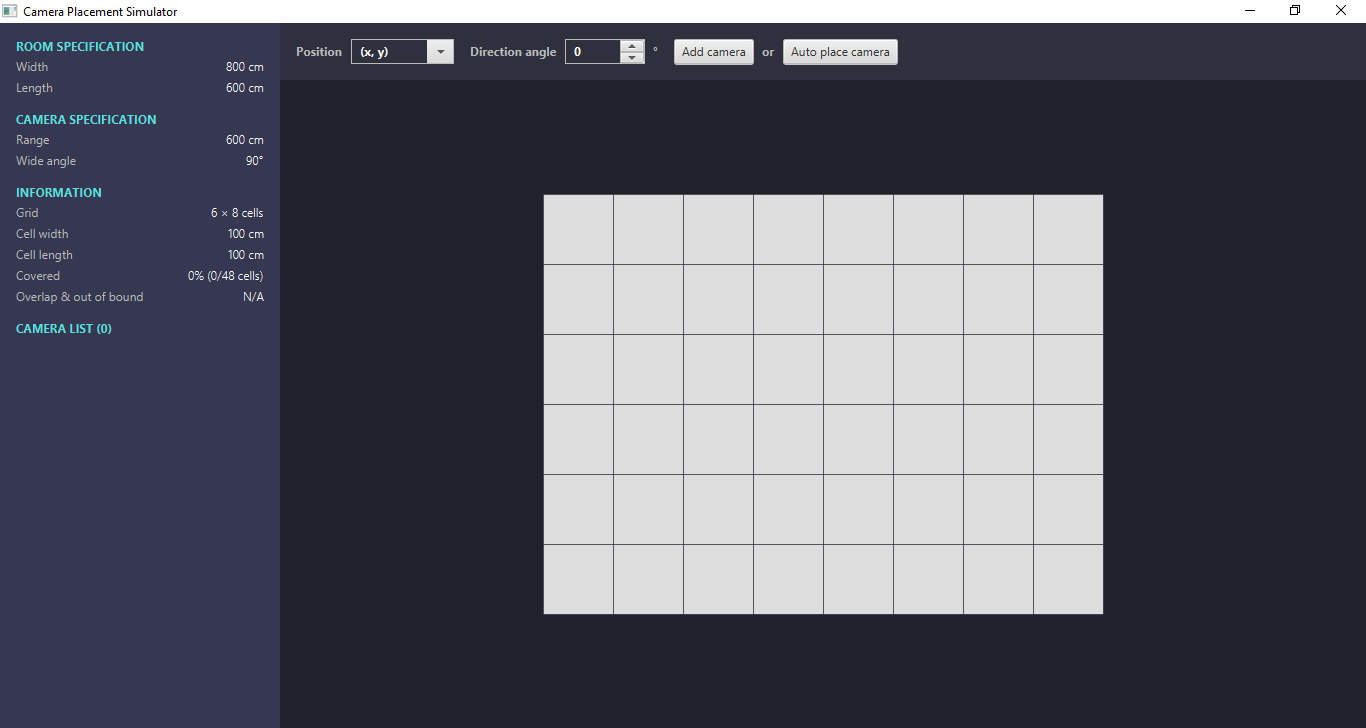
\includegraphics[scale=0.45]{ui_simulator}
%		\caption[Tampilan setelah pengisian masukan masalah]{Tampilan setelah pengisian masukan masalah}
%		\label{fig:testing_input_after}
%	\end{figure}
%	
%	Pada panel informasi, terdapat informasi masalah yang sesuai dengan masukan yang diberikan. Panel informasi dapat dilihat pada gambar~\ref{fig:testing_input_side_pane_after}.
%	
%	\begin{figure}[H]
%		\centering  
%		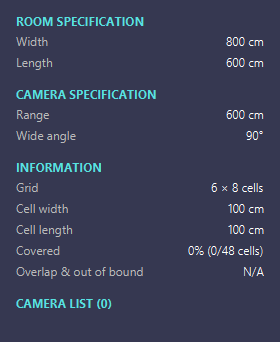
\includegraphics[scale=0.6]{testing_input_side_pane_after}
%		\caption[Tampilan panel informasi setelah pengisian masukan masalah]{Tampilan panel informasi setelah pengisian masukan masalah}
%		\label{fig:testing_input_side_pane_after}
%	\end{figure}	
%	
%	Hal ini menunjukkan bahwa proses memasukkan spesifikasi masalah telah berjalan sesuai dengan fungsinya. Dengan demikian, pengujian memasukkan spesifikasi masalah telah berhasil dilakukan.
%	
%	\item Pengujian: \textbf{Menambahkan Penempatan Kamera CCTV}\\
%	Pada pengujian ini, akan diuji apakah perangkat lunak dapat merespon penambahan penempatan kamera CCTV dengan memperbaharui panel informasi dan panel visualisasi. Pengujian dilakukan dengan memilih titik (0, 0) dan mengisi sudut \(315^\circ\) sebagai posisi dan sudut arah pandang kamera CCTV. Gambar~\ref{fig:testing_add_placement_top_pane} menunjukkan tampilan pada saat mengisi penempatan kamera CCTV.
%	
%	\begin{figure}[H]
%		\centering  
%		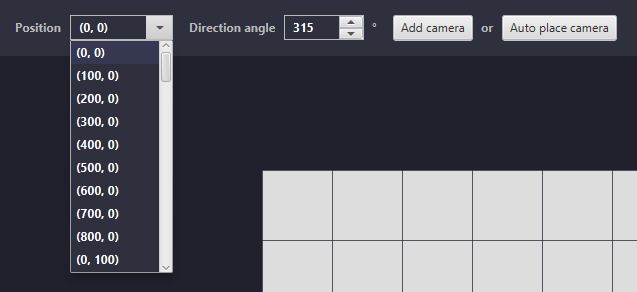
\includegraphics[scale=0.6]{testing_add_placement_top_pane}
%		\caption[Tampilan panel penambahan penempatan kamera CCTV]{Tampilan panel penambahan penempatan kamera CCTV}
%		\label{fig:testing_add_placement_top_pane}
%	\end{figure}
%	
%	 Setelah mengisi penempatan tersebut, tombol ''\textit{add camera}'' ditekan. Perangkat lunak merespon penambahan penempatan tersebut dengan memperbaharui panel informasi dan panel visualisasi seperti pada gambar~\ref{fig:testing_add_placement_side_pane_after} dan~\ref{fig:testing_add_placement_visualization_pane_after}. 
%	 
%	 \begin{figure}[H]
%		\centering  
%		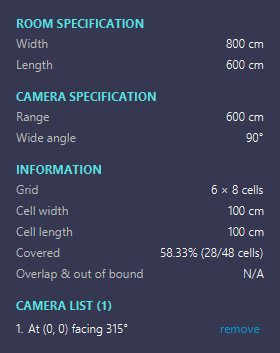
\includegraphics[scale=0.6]{testing_add_placement_side_pane_after}
%		\caption[Tampilan panel informasi setelah menambah penempatan kamera CCTV]{Tampilan panel informasi setelah menambah penempatan kamera CCTV}
%		\label{fig:testing_add_placement_side_pane_after}
%	\end{figure}
%	
%	\begin{figure}[H]
%		\centering  
%		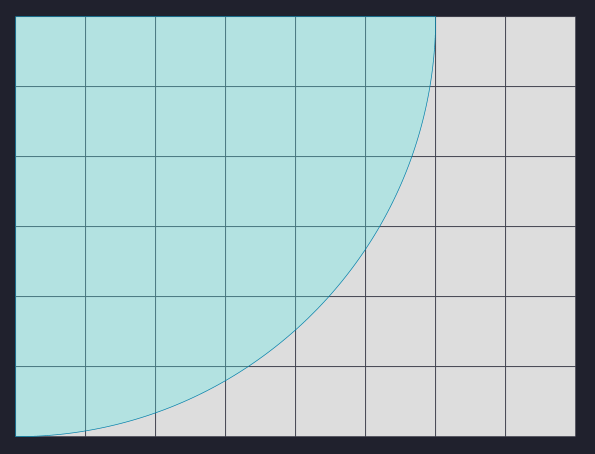
\includegraphics[scale=0.45]{testing_add_placement_visualization_pane_after}
%		\caption[Tampilan panel visualisasi setelah menambah penempatan kamera CCTV]{Tampilan panel visualisasi setelah menambah penempatan kamera CCTV}
%		\label{fig:testing_add_placement_visualization_pane_after}
%	\end{figure}
%	 
%	 Pada panel informasi bagian daftar penempatan kamera CCTV, terdapat baris baru bertuliskan ''\textit{At} (0, 0) \textit{facing} \(315^\circ\)'' yang menunjukkan penempatan pada titik (0, 0) dengan sudut arah pandang \(315^\circ\). Selain itu, informasi-informasi lainnya yang terdapat pada panel informasi juga telah diperbaharui. Pada panel visualisasi terdapat visualisasi objek kamera CCTV pada titik (0, 0) dengan sudut arah pandang \(315^\circ\). Hal ini menunjukkan bahwa penambahan penempatan kamera CCTV telah berhasil dilakukan sehingga proses menambahkan penempatan kamera CCTV dinyatakan berjalan sesuai dengan fungsinya. Dengan demikian, pengujian menambahkan penempatan kamera CCTV telah berhasil dilakukan.
%	
%	\item Pengujian: \textbf{Membuang Penempatan Kamera CCTV}\\
%	Pada pengujian ini akan diuji apakah perangkat lunak dapat merespon pembuangan penempatan kamera CCTV dengan memperbaharui panel informasi dan panel visualisasi penempatan kamera CCTV. Pengujian dilakukan dengan memilih penempatan pada titik (0, 0) dengan sudut arah pandang (\(315^\circ\)) sebagai penempatan yang akan dibuang. Pada penempatan tersebut, tombol ''\textit{remove}'' ditekan. Perangkat lunak merespon pembuangan penempatan tersebut dengan memperbaharui panel informasi dan panel visualisasi seperti pada gambar~\ref{fig:testing_remove_placement_information_pane_after} dan~\ref{fig:testing_remove_placement_visualization_pane_after}. 
%	
%	\begin{figure}[H]
%		\centering  
%		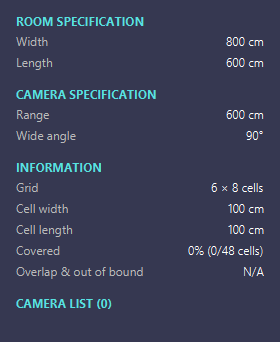
\includegraphics[scale=0.6]{testing_input_side_pane_after}
%		\caption[Tampilan panel informasi setelah membuang penempatan kamera CCTV]{Tampilan panel informasi setelah membuang penempatan kamera CCTV}
%		\label{fig:testing_remove_placement_information_pane_after}
%	\end{figure}
%	
%	\begin{figure}[H]
%		\centering  
%		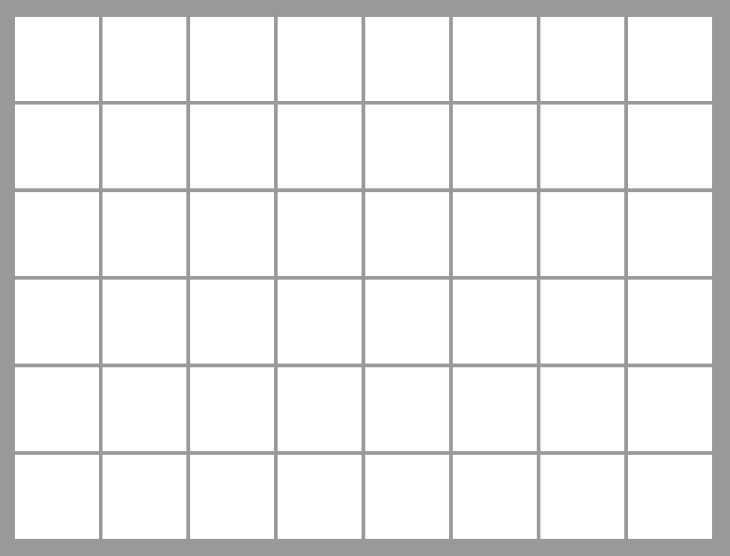
\includegraphics[scale=0.5]{testing_remove_placement_visualization_pane_after}
%		\caption[Tampilan panel visualisasi setelah membuang penempatan kamera CCTV]{Tampilan panel visualisasi setelah membuang penempatan kamera CCTV}
%		\label{fig:testing_remove_placement_visualization_pane_after}
%	\end{figure}	
%	
%	Pada panel informasi bagian daftar penempatan, tidak lagi ditemukan penempatan pada titik (0, 0) dengan sudut arah pandang \(315^\circ\). Pada panel visualisasi juga tidak lagi ditemukan visualisasi objek kamera CCTV pada titik (0, 0) dengan sudut arah pandang \(315^\circ\). Hal ini menunjukkan bahwa pembuangan penempatan kamera CCTV telah berhasil dilakukan sehingga proses membuang penempatan kamera CCTV dinyatakan berjalan sesuai dengan fungsinya. Dengan demikian, pengujian membuang penempatan kamera CCTV telah berhasil dilakukan.
%
%\end{itemize}

%\section{Pengujian Perangkat Lunak}
%Pada bagian ini akan dibahas pengujian yang bertujuan kebenaran metode penyelesaian masalah yang telah dibahas sebelumnya. Pada pemodelan masalah, telah dibahas pemodelan ruangan ke dalam bentuk grid point sehingga daerah dalam ruangan dimodelkan dalam bentuk cell-cell. Selain itu juga, telah dibahas bahwa cakupan kamera CCTV dinyatakan dalam bentuk kumpulan cell sehingga mencakup seluruh ruangan berarti sama dengan mencakup seluruh cell pada ruangan. Pemodelan masalah ini digunakan dalam metode penyelesaian masalah menggunakan teknik linear programming yang tujuannya adalah mencari penempatan-penempatan kamera CCTV yang berjumlah paling minimum yang mencakup seluruh ruangan. Sehingga tujuan dari pengujian ini adalah menguji apakah tujuan dari metode penyelesaian masalah tersebut telah tercapai.

%Pada pengujian ini akan dilakukan eksperimen-eksperimen untuk memastikan bahwa perangkat lunak dapat menyelesaikan permasalahan sesuai dengan tujuannya. Terdapat beberapa pengujian perangkat lunak yang dilakukan, yaitu:

%Pengujian perangkat lunak akan dilakukan dengan melakukan eksperimen-eksperimen, sehingga hasilnya dapat dianalisa. Eksperimen akan dibagi menjadi 2 bagian utama. Pada bagian pertama akan dilakukan eksperimen untuk menganalisa tingkat \textit{overlap} dan \textit{out of bound}. Bagian kedua akan dilakukan eksperimen untuk menganalisa jumlah kamera minimum.
%\section{Pengujian Eksperimental}
%Pada bagian ini akan dibahas pengujian yang dilakukan dengan eksperimen. Eksperimen yang dilakukan bertujuan untuk mendapatkan informasi mengenai korelasi masukan spesifikasi masalah dengan tingkat \textit{overlap} dan \textit{out of bound}. Pada setiap eksperimen, akan dijalankan proses pencarian minimum kamera CCTV untuk mendapatkan hasil yang dapat dianalisa. Gambar tampilan perangkat lunak untuk setiap eksperimen dapat dilihat pada bagian lampiran.
%
%\subsection{Eksperimen Ukuran Cell}
%Pada eksperimen ini akan dianalisa tingkat \textit{overlap} dan \textit{out of bound} terhadap ukuran cell. Eksperimen ini dilakukan sebanyak 3 kali dengan ukuran cell yang berbeda. Berikut ini merupakan spesifikasi masalah yang digunakan dalam eksperimen ini:
%\begin{enumerate}
%	\item Eksperimen pertama
%	\begin{itemize}
%		\item Lebar ruangan: 800 cm
%		\item Panjang ruangan: 600 cm
%		\item Jarak pandang kamera CCTV: 275 cm
%		\item Besar sudut pandang kamera CCTV: \(90^\circ\)
%		\item Ukuran cell: 100 cm
%	\end{itemize}
%		
%	\item Eksperimen kedua
%	\begin{itemize}
%		\item Lebar ruangan: 800 cm
%		\item Panjang ruangan: 600 cm
%		\item Jarak pandang kamera CCTV: 275 cm
%		\item Besar sudut pandang kamera CCTV: \(90^\circ\)
%		\item Ukuran cell: 50 cm
%	\end{itemize}
%		
%	\item Eksperimen ketiga
%	\begin{itemize}
%		\item Lebar ruangan: 800 cm
%		\item Panjang ruangan: 600 cm
%		\item Jarak pandang kamera CCTV: 275 cm
%		\item Besar sudut pandang kamera CCTV: \(90^\circ\)
%		\item Ukuran cell: 25 cm
%	\end{itemize}
%\end{enumerate}
%	
%Berdasarkan eksperimen yang dilakukan, didapatkan hasil sebagai berikut:
%\begin{enumerate}
%	\item Eksperimen pertama
%	\begin{itemize}
%		\item Tingkat \textit{overlap} dan \textit{out of bound}: 0\%
%	\end{itemize}
%	
%	\item Eksperimen kedua
%	\begin{itemize}
%		\item Tingkat \textit{overlap} dan \textit{out of bound}: 14.58\%
%	\end{itemize}
%	
%	\item Eksperimen ketiga
%	\begin{itemize}
%		\item Tingkat \textit{overlap} dan \textit{out of bound}: 25\%
%	\end{itemize}
%\end{enumerate}
%
%Berdasarkan hasil tersebut, didapatkan bahwa pemodelan menggunakan cell yang berukuran lebih kecil akan menghasilkan efektivitas yang lebih baik, yakni tingkat \textit{overlap} dan \textit{out of bound} yang lebih kecil.
%Berdasarkan hasil tersebut, didapatkan bahwa semakin besar ukuran terbesar cell, maka tingkat \textit{overlap} dan \textit{out of bound} akan semakin besar.
%Hal ini disebabkan karena semakin kecil ukuran cell, maka akurasi ketercakup cell semakin besar, sehingga tingkat \textit{overlap} dan \textit{out of bound} semakin besar.

%\subsection{Eksperimen Rasio Sisi Terpendek Ruangan dengan Jarak Pandang Kamera CCTV}
%Pada eksperimen ini akan dianalisa tingkat \textit{overlap} dan \textit{out of bound} terhadap rasio antara sisi terpendek ruangan dengan jarak pandang kamera CCTV. Eksperimen ini dilakukan sebanyak 4 kali dengan jarak pandang kamera CCTV yang berbeda sehingga didapatkan rasio yang berbeda. Berikut ini merupakan spesifikasi masalah yang digunakan dalam eksperimen ini:
%
%\begin{enumerate}
%	\item Eksperimen pertama
%	\begin{itemize}
%		\item Lebar ruangan: 400 cm
%		\item Panjang ruangan: 300 cm
%		\item Jarak pandang kamera CCTV: 300 cm
%		\item Besar sudut pandang kamera CCTV: \(90^\circ\)
%		\item Ukuran cell: 25 cm
%		\item Rasio \(\frac{\text{sisi terpendek ruangan}}{\text{jarak pandang kamera CCTV}}\) = 1
%	\end{itemize}
%	
%	\item Eksperimen kedua
%	\begin{itemize}
%		\item Lebar ruangan: 400 cm
%		\item Panjang ruangan: 300 cm
%		\item Jarak pandang kamera CCTV: 150 cm
%		\item Besar sudut pandang kamera CCTV: \(90^\circ\)
%		\item Ukuran cell: 25 cm
%		\item Rasio \(\frac{\text{sisi terpendek ruangan}}{\text{jarak pandang kamera CCTV}}\) = 2
%	\end{itemize}
%	
%	\item Eksperimen ketiga
%	\begin{itemize}
%		\item Lebar ruangan: 400 cm
%		\item Panjang ruangan: 300 cm
%		\item Jarak pandang kamera CCTV: 100 cm
%		\item Besar sudut pandang kamera CCTV: \(90^\circ\)
%		\item Ukuran cell: 25 cm
%		\item Rasio \(\frac{\text{sisi terpendek ruangan}}{\text{jarak pandang kamera CCTV}}\) = 3
%	\end{itemize}
%	
%	\item Eksperimen keempat
%	\begin{itemize}
%		\item Lebar ruangan: 400 cm
%		\item Panjang ruangan: 300 cm
%		\item Jarak pandang kamera CCTV: 75 cm
%		\item Besar sudut pandang kamera CCTV: \(90^\circ\)
%		\item Ukuran cell: 25 cm
%		\item Rasio \(\frac{\text{sisi terpendek ruangan}}{\text{jarak pandang kamera CCTV}}\) = 4
%	\end{itemize}
%\end{enumerate}
%
%Berdasarkan eksperimen yang dilakukan, didapatkan hasil sebagai berikut:
%\begin{enumerate}
%	\item Eksperimen pertama
%	\begin{itemize}
%		\item Tingkat \textit{overlap} dan \textit{out of bound}: 75\%
%	\end{itemize}
%		
%	\item Eksperimen kedua
%	\begin{itemize}
%		\item Tingkat \textit{overlap} dan \textit{out of bound}: 16.67\%
%	\end{itemize}
%	
%	\item Eksperimen ketiga
%	\begin{itemize}
%		\item Tingkat \textit{overlap} dan \textit{out of bound}: 8.33\%
%	\end{itemize}
%	\item Eksperimen keempat
%	\begin{itemize}
%		\item Tingkat \textit{overlap} dan \textit{out of bound}: 0\%
%	\end{itemize}
%\end{enumerate}
%Berdasarkan hasil tersebut, didapatkan bahwa semakin besar rasio sisi terpendek ruangan dengan jarak pandang kamera CCTV, maka tingkat \textit{overlap} dan \textit{out of bound} akan semakin kecil.
%
%\subsection{Eksperimen Besar Sudut Pandang Kamera CCTV}
%Pada eksperimen ini akan dianalisa tingkat \textit{overlap} dan \textit{out of bound} terhadap besar sudut pandang kamera CCTV. Eksperimen ini dilakukan sebanyak 4 kali dengan besar sudut pandang kamera CCTV yang berbeda. Berikut ini merupakan spesifikasi masalah yang digunakan dalam eksperimen ini:
%
%\begin{enumerate}
%	\item Eksperimen pertama
%	\begin{itemize}
%		\item Lebar ruangan: 400 cm
%		\item Panjang ruangan: 300 cm
%		\item Jarak pandang kamera CCTV: 135 cm
%		\item Besar sudut pandang kamera CCTV: \(90^\circ\)
%		\item Ukuran cell: 25 cm
%	\end{itemize}
%	
%	\item Eksperimen kedua
%	\begin{itemize}
%		\item Lebar ruangan: 400 cm
%		\item Panjang ruangan: 300 cm
%		\item Jarak pandang kamera CCTV: 135 cm
%		\item Besar sudut pandang kamera CCTV: \(75^\circ\)
%		\item Ukuran cell: 25 cm
%	\end{itemize}
%	
%	\item Eksperimen ketiga
%	\begin{itemize}
%		\item Lebar ruangan: 400 cm
%		\item Panjang ruangan: 300 cm
%		\item Jarak pandang kamera CCTV: 135 cm
%		\item Besar sudut pandang kamera CCTV: \(60^\circ\)
%		\item Ukuran cell: 25 cm
%	\end{itemize}
%	
%	\item Eksperimen keempat
%	\begin{itemize}
%		\item Lebar ruangan: 400 cm
%		\item Panjang ruangan: 300 cm
%		\item Jarak pandang kamera CCTV: 135 cm
%		\item Besar sudut pandang kamera CCTV: \(45^\circ\)
%		\item Ukuran cell: 25 cm
%	\end{itemize}
%\end{enumerate}
%
%Berdasarkan eksperimen yang dilakukan, didapatkan hasil sebagai berikut:
%\begin{enumerate}
%	\item Eksperimen pertama
%	\begin{itemize}
%		\item Tingkat \textit{overlap} dan \textit{out of bound}: 14.58\%
%	\end{itemize}
%		
%	\item Eksperimen kedua
%	\begin{itemize}
%		\item Tingkat \textit{overlap} dan \textit{out of bound}: 18.75\%
%	\end{itemize}
%	
%	\item Eksperimen ketiga
%	\begin{itemize}
%		\item Tingkat \textit{overlap} dan \textit{out of bound}: 16.15\%
%	\end{itemize}
%	\item Eksperimen keempat
%	\begin{itemize}
%		\item Tingkat \textit{overlap} dan \textit{out of bound}: 8.33\%
%	\end{itemize}
%\end{enumerate}
%Berdasarkan hasil tersebut, tidak ditemukan adanya korelasi besar sudut pandang kamera CCTV terhadap tingkat \textit{overlap} dan \textit{out of bound}.